\section{Experiments}
\label{sec:experiments}

\subsection{Protocol}

Everything in this section was produced by \file{paper/scripts/} in one
sitting, on the machine described in \cref{app:repro}, from the checkpoints
\file{move\_ctc\_spd\_s0.pt} and \file{move\_ctc\_spd\_s1.pt} unless stated
otherwise. Rules, each of which has cost this project a wrong conclusion at
some point:

\begin{enumerate}[leftmargin=1.4em,itemsep=2pt]
\item \textbf{Both seeds, always.} The two-seed spread on this metric is
0.5--3 points and several historical ``improvements'' were smaller.
\item \textbf{Never pool a mean over moves when the claim is about
sessions.} The headline is a mean of per-session accuracies; a long solve
must not dominate a short one. Pooled numbers are reported separately where
they differ.
\item \textbf{Split by lighting regime, never pooled.} The pooled
distribution is bimodal and the pooled mean describes nothing.
\item \textbf{Re-run the baseline in the same sitting.} No number here is
compared against a value recalled from a document.
\item \textbf{Held-out means held out of training \emph{and} validation}
(\cref{sec:holdout-hygiene}).
\item \textbf{Resample sessions, not moves.} Confidence intervals are
bootstrapped over sessions ($20{,}000$ resamples), because the quantity
being estimated is ``what would this model score on a new session'', and
moves within a session are strongly dependent --- the $16\times$
per-session spread in miss rate \emph{is} that dependence. Resampling moves
would give intervals several times too narrow.
\item \textbf{Compare rungs pairwise.} Every ablation rung is scored on the
same \NPaired\ sessions, so the statistic is the mean per-session
\emph{difference}, tested with an exact sign test (no distributional
assumption at this $n$).
\end{enumerate}

The metric is per-move accuracy under Needleman--Wunsch alignment against the
camera-frame BLE word: alignment, not index-by-index comparison, because one
dropped move shifts every later index and a positional comparison would read
a single miss as ${\sim}25$ errors. The alignment's three non-match
operations are exactly the three failure modes: \emph{miss} (recall),
\emph{phantom} (precision), \emph{substitution} (naming). Move error rate
(Levenshtein distance over $|{\rm truth}|$) is reported alongside because it
charges phantoms, which accuracy does not.

\subsection{Main result: raw recognition}
\label{sec:main-results}

\begin{table}[t]
\centering\small
\caption{Raw CTC recognition on the never-seen holdout, mean of per-session
accuracies. The CTC ceiling column is the structural limit from
\cref{sec:ctc-bg} --- same-class onset pairs within two frames, which no
amount of training removes.}
\label{tab:main}
\begin{tabular}{@{}llrrrrr@{}}
\toprule
take type & regime & $n$ & moves & seed 0 & seed 1 & CTC ceiling \\
\midrule
solve & daytime & 9 & 1003 & 91.2\% & 90.2\% & 98.1\% \\
solve & evening & 5 & 552 & 85.2\% & 90.0\% & 99.1\% \\
solve & all & 14 & 1555 & 89.0\% & 90.2\% & 98.5\% \\
\midrule
scramble & daytime & 9 & 186 & 97.2\% & 97.2\% & 100.0\% \\
scramble & evening & 5 & 100 & 97.0\% & 96.0\% & 100.0\% \\
scramble & all & 14 & 286 & 97.1\% & 96.8\% & 100.0\% \\
\bottomrule
\end{tabular}

\end{table}

On \NHoldoutSolves\ free solves (\NHoldoutMoves\ turns) no checkpoint has
seen, per-move accuracy is \RawDaySA\%/\RawDaySB\% daytime and
\RawEveSA\%/\RawEveSB\% evening by seed, against a structural CTC ceiling
of \CTCCeilingHoldout\%. Averaging the seeds and bootstrapping over
sessions, that is \CIDayMean\% [\CIDayLo, \CIDayHi] daytime and
\CIEveMean\% [\CIEveLo, \CIEveHi] evening --- intervals wide enough that
the two regimes overlap, which is worth keeping in mind every time this
report calls the evening gap large.
On the \NHoldoutScrambles\ prescribed-scramble
takes --- 20 slow, well-separated moves each --- it is \ScrSA\%/\ScrSB\%.
The gap between those two lines is the whole difficulty of the problem: the
same model, the same room, the same cube, differing only in that a solve is
long, fast and crowded.

\Cref{fig:persession} shows the per-session spread, which is the number that
actually matters for a product because a user experiences one solve, not a
mean. The worst held-out session reads \RawMinSA\%; the best reads over
97\%. That is a $16\times$ spread in miss rate across sessions, on
\emph{identical weights} --- and it is the strongest single piece of evidence
that the binding constraint is data coverage, not model capacity. A model
short on capacity is short everywhere.

\begin{figure}[t]
\centering
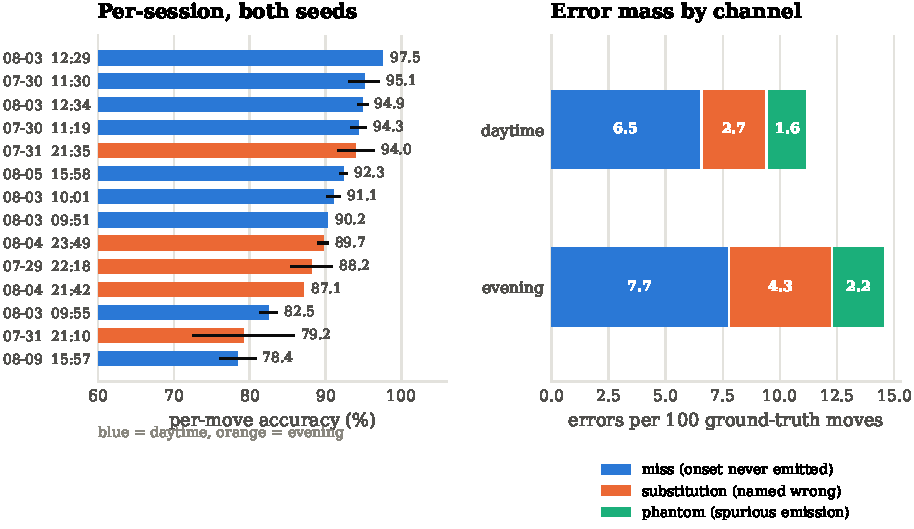
\includegraphics[width=\linewidth]{figures/fig_persession.pdf}
\caption{Left: per-session accuracy on the held-out set; bar is the two-seed
mean, black line the spread. Right: where the error mass goes. Misses
dominate in both lighting regimes.}
\label{fig:persession}
\end{figure}

\paragraph{Decoding choice.} Prefix beam search over the posteriorgram beats
best-path (greedy) decoding by \GreedyGap\ points on average --- small, but
consistent, and free.

\paragraph{Error composition.} Pooled over the holdout and both seeds:
\MissRate\ misses, \SubRate\ substitutions and \PhantomRate\ phantoms per 100
ground-truth moves. As shares of total error mass that is
\MissShare\% miss, \SubShare\% substitution, \PhantomShare\% phantom. The
implication runs through the rest of this report: \textbf{the pipeline's
dominant failure is not naming a move wrongly, it is not seeing it at all},
and the group decoder's strongest channel is the smallest one.

\subsection{How much of that number is generalisation?}
\label{sec:ladder}

\begin{figure}[t]
\centering
\begin{minipage}{0.47\linewidth}
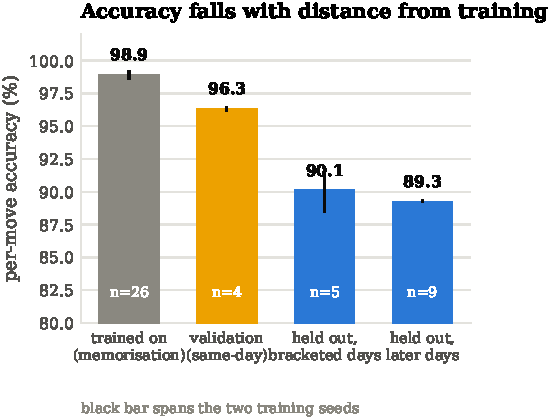
\includegraphics[width=\linewidth]{figures/fig_ladder.pdf}
\end{minipage}\hfill
\begin{minipage}{0.5\linewidth}
\small
The same weights, scored on four tiers of increasing distance from training.
The \LadderValMinusHeld-point drop from validation to genuinely-unseen
sessions is the size of the error a same-day validation split makes. Note
that ``bracketed'' days
(held out, but sandwiched between training days) score no better than
``later'' days --- so this is not primarily temporal extrapolation, it is
simply \emph{unseen session}.
\end{minipage}
\caption{Holdout proximity ladder. Bars are the two-seed mean; the black
line spans the seeds.}
\label{fig:ladder}
\end{figure}

Accuracy falls monotonically with distance from training:
\LadderTrain\% on sessions the checkpoints trained on, \LadderVal\% on the
same-day validation sessions that chose the stopping epoch, and
\LadderHeld\% on sessions never seen in any capacity --- a
\LadderTrainMinusHeld-point spread.

Two readings follow.

\begin{enumerate}[leftmargin=1.4em,itemsep=3pt]
\item \textbf{Validation MER cannot rank interventions here.} It sits
\LadderTrainMinusVal\ points below train and \LadderValMinusHeld\ above the
honest holdout, on same-day neighbours. \cref{sec:ablation} shows two interventions that validation
called flat and the holdout calls large.
\item \textbf{The repository's published numbers are optimistic, and by a
knowable amount.} Scored under this report's harness, the eight sessions the
repository calls held out give 89.9\%/92.7\% by seed; the strictly-defined
14 give \RawAllSA\%/\RawAllSB\%. The difference is small, but it is in the
direction the selection predicts, and the eight included two validation
sessions.
\end{enumerate}

\subsection{The ablation ladder}
\label{sec:ablation}

\begin{table}[t]
\centering\small
\caption{Five checkpoint generations, two seeds each, all scored on the
\emph{same} \NHoldoutSolves\ never-seen solves. ``train'' is the number of
sessions that configuration trained on.}
\label{tab:ablation}
\begin{tabular}{@{}lrrrr@{}}
\toprule
configuration & train & daytime & evening & all \\
\midrule
peak-pick (joint) & 38 & 78.2\% & 63.9\% & 73.1\% \\
CTC & 38 & 81.9\% & 61.0\% & 74.4\% \\
CTC + photo-aug & 38 & 82.6\% & 73.3\% & 79.3\% \\
CTC + photo-aug + 6 sessions & 44 & 86.0\% & 78.7\% & 83.4\% \\
CTC + photo + speed aug & 44 & 90.7\% & 87.6\% & 89.6\% \\
\bottomrule
\end{tabular}

\end{table}

\begin{figure}[t]
\centering
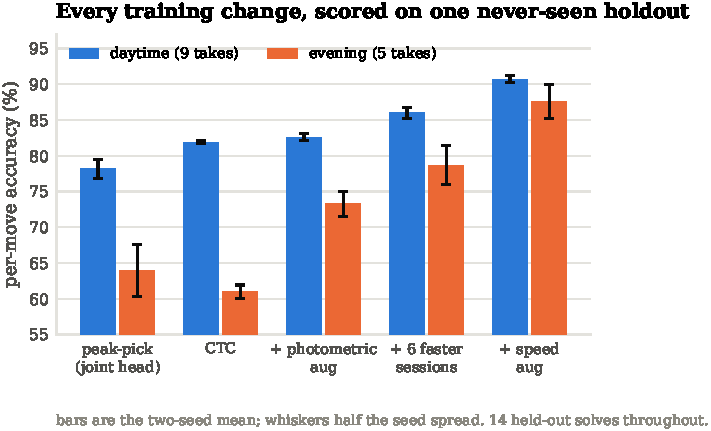
\includegraphics[width=0.92\linewidth]{figures/fig_ablation.pdf}
\caption{Each rung adds exactly one thing to the rung below it. The holdout
is intersected across all ten checkpoints, so no rung is scored on a session
any rung has seen.}
\label{fig:ablation}
\end{figure}

This is the first time these five configurations have been comparable: each
was historically evaluated on whatever holdout existed that week. Because
every rung is scored on the same \NPaired\ sessions, the rungs can be
compared \emph{pairwise}, which is far more powerful than comparing two
means:

\begin{center}\small
\begin{tabular}{@{}lrrr@{}}
\toprule
step & $\Delta$ accuracy & 95\% CI & sign test \\
\midrule
peak-picking $\to$ CTC & \DCtcVsPeak &
  [\DCtcVsPeakLo, \DCtcVsPeakHi] & $p = $ \DCtcVsPeakP \\
$+$ widened photometric augmentation & \DPhotoAug &
  [\DPhotoAugLo, \DPhotoAugHi] & $p = $ \DPhotoAugP \\
$+$ six more (faster) training sessions & \DMoreSessions &
  [\DMoreSessionsLo, \DMoreSessionsHi] & $p$ \DMoreSessionsP \\
$+$ speed augmentation & \DSpeedAug &
  [\DSpeedAugLo, \DSpeedAugHi] & $p$ \DSpeedAugP \\
\midrule
first rung $\to$ last rung & \DTotal &
  [\DTotalLo, \DTotalHi] & $p$ \DMoreSessionsP \\
\bottomrule
\end{tabular}
\end{center}

\begin{description}[leftmargin=1.2em,style=nextline,itemsep=4pt]
\item[Peak-picking $\to$ CTC: \DCtcVsPeak\ points, \emph{not significant}
($p = $ \DCtcVsPeakP, \DCtcVsPeakBetter\ sessions better,
\DCtcVsPeakWorse\ worse).] This is the project's headline architectural
change and on this holdout it cannot be distinguished from noise. What
\emph{does} change dramatically is the error composition: substitutions and
phantoms fall sharply while misses rise --- CTC trades ``fires and names it
wrong'' for ``does not fire''. Whether that is an improvement depends on the
consumer: for the group decoder it is \emph{worse}, because substitutions
are its cheap channel and misses its expensive one; for the count gate it is
roughly neutral. The defensible case for CTC is not this delta, it is that
CTC removes the constant-tuning failure mode of \cref{sec:peakpick} and that
its advantage grows with every later rung.
\item[Widened photometric augmentation: \DPhotoAug\ points, marginal
($p = $ \DPhotoAugP).] Concentrated almost entirely in the evening
(\PhotoAugEveningGain\ there, \PhotoAugDaytimeGain\ daytime), which is why
the pooled test is weak: it is a large effect on 5 of \NPaired\ sessions.
This is the synthetic substitute for evening data and within its regime it
works.
\item[Six more (faster) training sessions: \DMoreSessions\ points
($p$ \DMoreSessionsP).] Significant, and unglamorous: the corpus was stale
relative to how fast the solver had become.
\item[Speed augmentation: \DSpeedAug\ points ($p$ \DSpeedAugP),
\DSpeedAugBetter\ of \NPaired\ sessions better.] \textbf{The largest and
most significant single accuracy intervention in the project's history ---
and it was recorded as costing nothing.} It was introduced to stop the count
gate under-reading fast solves, judged on validation MER (which was flat,
correctly: the validation sessions are slow), and shipped as a neutral
change.
\end{description}

\begin{keybox}
The pattern is the result. \textbf{The two \emph{data} interventions are
significant and the two \emph{method} interventions are not} --- and both
data interventions were invisible to the validation metric used to judge
them, for the same structural reason: the validation split is
same-day-adjacent and therefore drawn from the regime that already worked. A
holdout is not a formality; on this corpus it is the only instrument that
can see the interventions that matter.
\end{keybox}

Total across the ladder: \DTotal\ points [\DTotalLo, \DTotalHi] on the same
never-seen sessions.

\subsection{Error analysis}
\label{sec:erroranalysis}

\begin{figure}[t]
\centering
\begin{minipage}{0.47\linewidth}
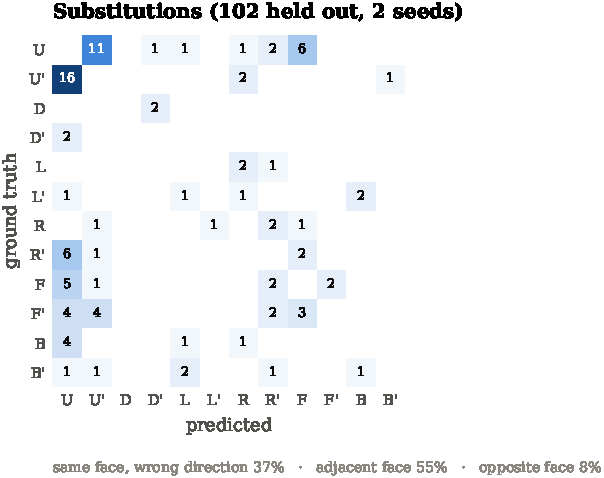
\includegraphics[width=\linewidth]{figures/fig_confusion.pdf}
\end{minipage}\hfill
\begin{minipage}{0.47\linewidth}
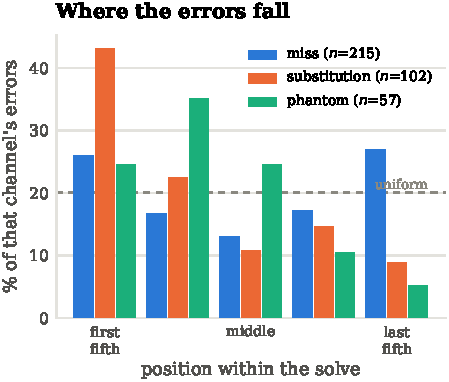
\includegraphics[width=\linewidth]{figures/fig_errpos.pdf}
\end{minipage}
\caption{Left: the \NSubTotal\ substitutions on the holdout, both seeds.
Right: where each error channel falls within a solve.}
\label{fig:erroranalysis}
\end{figure}

\paragraph{Substitutions are mostly adjacent-face, not direction errors.}
\SubAdjacent\% name a face adjacent to the true one, \SubInverse\% get the
face right and the direction wrong, \SubOpposite\% name the opposite face.
This settles a question the project re-litigated repeatedly: on
\emph{in-distribution} data the residual error is direction confusion (the
hard case that survives when everything else works), but in the live long-solve
regime it is a more basic wrong-face error. The held-out measurement here
agrees with the live regime, which is the one that matters. An architecture
change that models time more richly targets the \SubInverse\% channel, not
the \SubAdjacent\% one.

\paragraph{There is a prediction bias toward the U layer.}
\PredUShare\% of all substitution \emph{predictions} are \wca{U} or \wca{U'},
against $\tfrac{2}{12}=17$\% under a uniform prior. The U layer is the most
frequent class in CFOP by a wide margin, and the model falls back on it when
unsure --- classic prior collapse, and a candidate for class-balanced
training or a logit prior correction. Not yet tried.

\paragraph{Errors are strongly non-uniform through a solve, and each channel
has its own shape.} \SubFirstFifth\% of substitutions fall in the first
fifth of the solve against \SubLastFifth\% in the last --- more than double
the uniform 20\%. Phantoms are similarly front-loaded
(\PhanFirstFifth\% vs \PhanLastFifth\%). Misses are the opposite shape:
roughly U-distributed, \MissFirstFifth\% at the start and
\MissLastFifth\% at the end with a trough in the middle.

The interpretation is CFOP's phase structure. The opening --- inspection,
cross, first F2L pair --- is where the cube is rotated and regripped most,
which is precisely the motion that looks like a turn without being one; that
produces both wrong names and spurious detections. The last fifth is the
last layer: fast, memorised, heavily crowded algorithm execution, where the
failure is not seeing turns at all.

This matters for the decoder. Its endpoint constraint is weakest exactly
where substitutions cluster (the beginning, dozens of moves from the only
anchor) and strongest where misses cluster (the end) --- but misses are the
channel it cannot cheaply repair. The two distributions are almost
maximally unhelpful to it.

\subsection{The truth frame is worth measuring}
\label{sec:frame-result}

Scoring the identical predictions against cube-frame truth (what the smart
cube reports, and what every harness in the repository still uses) versus
camera-frame truth (what a vision model can possibly predict,
\cref{sec:labelframe}):

\begin{center}\small
\begin{tabular}{@{}lrr@{}}
\toprule
scored over & cube-frame truth & camera-frame truth \\
\midrule
the three slice-bearing held-out sessions & \FrameCubeSlice\% &
\FrameCamSlice\% \\
the whole held-out set & \FrameCubeAll\% & \FrameCamAll\% \\
\bottomrule
\end{tabular}
\end{center}

\FrameGainSlice\ points where it applies, \FrameGainAll\ diluted over the
holdout. Small --- but it is a systematic bias against the model, it is free
to fix, and it is exactly the kind of thing that erodes confidence in
everything else in a paper when a reviewer finds it.

\subsection{The group decode and the falsifiability sweep}
\label{sec:decode-results}
\label{sec:falsifiability}

\begin{table}[t]
\centering\small
\caption{Group-theoretic decode, both seeds, on every held-out free solve.
$\Delta$ is post-decode minus raw. ``decoys accepted'' counts, out of eight
per session (four false claims $\times$ two seeds), how many wrong start
states the decoder found a valid story for. $\dagger$ marks sessions
containing a middle slice, where the decoder's cube-frame model and the
recogniser's camera-frame output are known to disagree
(\cref{sec:labelframe}).}
\label{tab:decode}
\begin{tabular}{@{}lrrrccc@{}}
\toprule
session & raw & post & $\Delta$ & verified & exact & decoys accepted \\
\midrule
07-29\,22:18$^{\dagger}$ & 86.8\% & 85.9\% & -1.0 & 0/2 & 0/2 & 0/8 \\
07-30\,11:19 & 94.3\% & 94.8\% & +0.5 & 0/2 & 0/2 & 0/8 \\
07-30\,11:30$^{\dagger}$ & 93.6\% & 93.6\% & +0.0 & 0/2 & 0/2 & 0/8 \\
07-31\,21:10 & 79.2\% & 79.2\% & +0.0 & 0/2 & 0/2 & 0/8 \\
07-31\,21:35 & 94.0\% & 93.1\% & -0.9 & 0/2 & 0/2 & 0/8 \\
08-03\,09:51 & 90.2\% & 89.6\% & -0.6 & 0/2 & 0/2 & 0/8 \\
08-03\,09:55$^{\dagger}$ & 78.9\% & 79.3\% & +0.4 & 0/2 & 0/2 & 0/8 \\
08-03\,10:01 & 91.1\% & 91.1\% & +0.0 & 0/2 & 0/2 & 0/8 \\
08-03\,12:29 & 97.5\% & 97.5\% & +0.0 & 0/2 & 0/2 & 0/8 \\
08-03\,12:34 & 94.9\% & 94.9\% & +0.0 & 0/2 & 0/2 & 0/8 \\
08-04\,21:42 & 87.1\% & 87.1\% & +0.0 & 0/2 & 0/2 & 0/8 \\
08-04\,23:49 & 89.7\% & 89.7\% & +0.0 & 0/2 & 0/2 & 0/8 \\
08-05\,15:58 & 92.3\% & 92.7\% & +0.4 & 0/2 & 0/2 & 0/8 \\
08-09\,15:57 & 78.4\% & 78.4\% & +0.0 & 0/2 & 0/2 & 0/8 \\
\bottomrule
\end{tabular}

\end{table}

\begin{figure}[t]
\centering
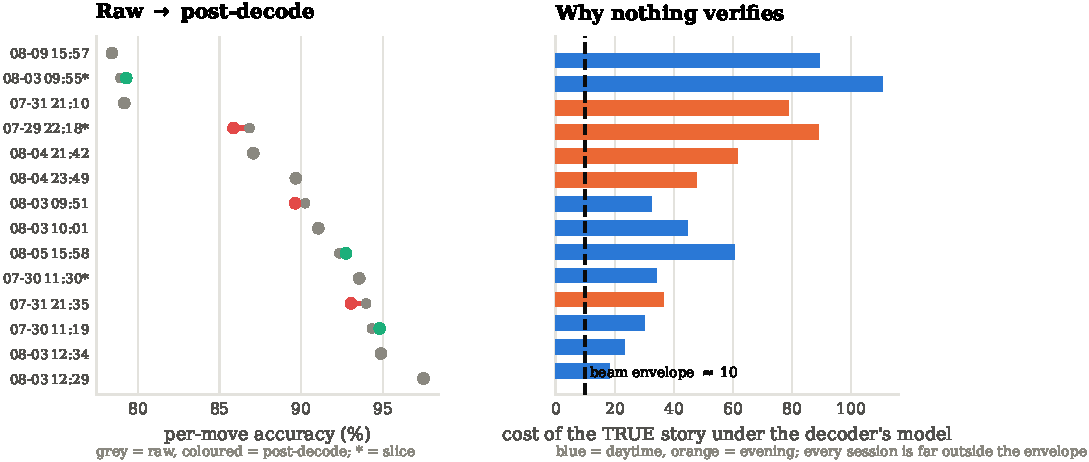
\includegraphics[width=\linewidth]{figures/fig_decode.pdf}
\caption{Left: what the group decode does to each session's accuracy.
Right: the falsifiability sweep --- the fraction of claims the decoder found
a solving story for, when the claim is true and when it is deliberately
wrong by 1, 2 or 4 quarter turns or entirely fabricated.}
\label{fig:decode}
\end{figure}

\begin{figure}[t]
\centering
\begin{minipage}{0.46\linewidth}
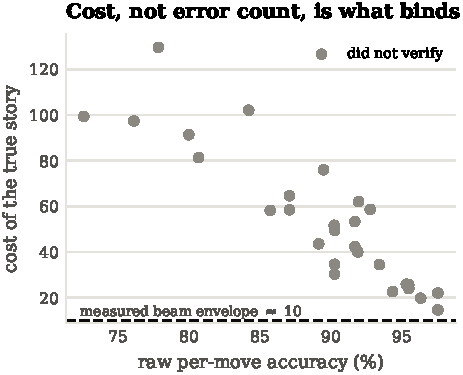
\includegraphics[width=\linewidth]{figures/fig_cliff.pdf}
\end{minipage}\hfill
\begin{minipage}{0.5\linewidth}\small
The decode's binding constraint is the \emph{cost} of the true story under
the model, not the number of errors in it. A story costing ${\sim}6$ survives
90 onsets at the deployed beam; one costing ${\sim}10$ does not, and every
insertion is a flat 4.0. On this holdout the cheapest true story costs
\MinGtPathCost\ and the median costs \MedGtPathCost\ --- every session is
outside the envelope, which is why the scatter has no verified points in it
at all.
\end{minipage}
\caption{Why the decode is all-or-nothing, and why on this holdout it is
uniformly ``nothing''.}
\label{fig:cliff}
\end{figure}

\textbf{The decode contributes nothing measurable on this holdout.} On the
\DecodeNonSliceN\ slice-free held-out solves it moves per-move accuracy from
\DecodeRaw\% to \DecodePost\% --- \DecodeGain\ points --- and it verifies
\DecodeVerified\ of \DecodeTrials\ session-seed pairs. Twenty of the 28
session-seed pairs are unchanged to three decimal places; of the eight that
move, four improve and four get \emph{worse}.

That is a substantially weaker result than the repository's ${\sim}+1.2$
points daytime, and the difference is not a contradiction --- it is the
holdout. The older figure was measured on a set whose sessions included
several with true-story costs near the beam's envelope; this holdout has
none. Which is exactly the prediction \cref{sec:decode-limits} makes: the
decode is worth about a point where it closes and nothing where it does not,
so a holdout two points harder collapses its contribution to zero.

\paragraph{The mechanism, restated with the numbers.} The endpoint
constraint is global and terminal. The cheapest true story on this holdout
costs \MinGtPathCost\ against an envelope of ${\sim}10$, and the median costs
\MedGtPathCost. At \MissShare\% miss-dominated error, each missing move
charges a flat $C_{\rm ins} = 4.0$ with no posterior evidence to offset it,
so a session with even five misses is already outside the envelope before
any naming error is counted. The sessions that most need repair are
precisely the ones whose repair is unaffordable.

\paragraph{Beam budget.} These runs use the deployed first-pass beam of
4000 without the production retry at $4\times$. That is a compute
concession, and it is checkable rather than assumed: a wider beam searches
the same cost landscape, and with the cheapest true story at
\MinGtPathCost\ there is nothing within the envelope for it to find. It
could in principle change a \emph{best-effort} story slightly; that is
untested here and is the one caveat on the \DecodeGain-point figure.

\paragraph{Slice sessions fail structurally, not statistically.} The
$\dagger$ sessions carry the highest costs relative to their raw accuracy,
because the model emits camera-frame move names into a decoder whose cube
model is centre-relative. This is a known, unfixed defect; the machinery to
handle it (persistent orientation state in the beam) exists and is disabled
on a premise --- ``the recorded sessions hold one orientation throughout'' ---
that these sessions falsify.

\paragraph{Falsifiability, and why this run cannot speak to it.}
\DecoyAccepted\ of \DecoyTried\ deliberately false claims were accepted.
\textbf{That is not a security result and must not be reported as one},
because the same decoder also rejected all \DecodeTrials\ \emph{true}
claims. A verifier that rejects everything has perfect specificity and zero
sensitivity; the sweep is uninformative when the true-positive rate is zero.

Two things do survive from it. First, the operational statement: at the
deployed beam nothing spurious was accepted. Second, and more usefully, the
constructive bound of \cref{eq:decoybound} still applies --- a valid story
for a $d$-move-off claim provably exists at $c(W) + 4d$, so any rejection
here is the search failing to find a story that is known to be there, not
the cost model ruling it out. A meaningful falsifiability measurement
requires sessions whose true claims verify, and this holdout has none. That
is a reason to record easier sessions for that specific test, not a reason
to quote 0/\DecoyTried.

\subsection{The count gate}
\label{sec:anticheat-results}

\begin{figure}[t]
\centering
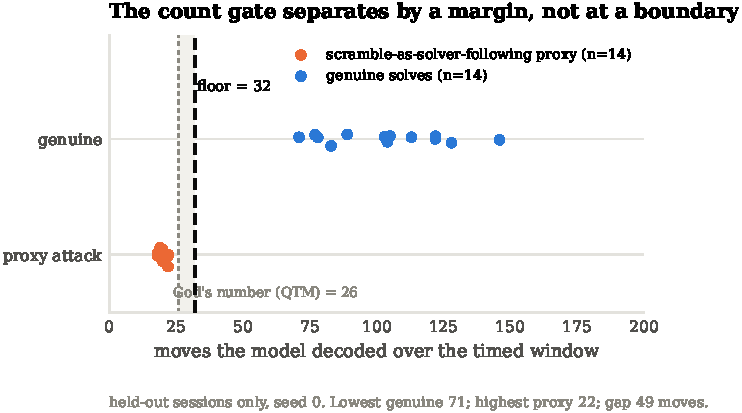
\includegraphics[width=0.92\linewidth]{figures/fig_anticheat.pdf}
\caption{Decoded move count on held-out sessions. Genuine solves and
scramble-as-solver-following proxies do not merely fall on opposite sides of
the threshold --- they are separated by \ACGapSA\ moves with the threshold
inside the gap.}
\label{fig:anticheat}
\end{figure}

On the strict holdout: \ACVerifiedSA/\ACSolves\ and
\ACVerifiedSB/\ACSolves\ genuine solves verified with zero false
disqualifications on either seed, and \ACCaughtSA/\ACProxies\ and
\ACCaughtSB/\ACProxies\ proxy attacks caught on either seed. The lowest
genuine solve reads \ACLowestLegit\ moves; the highest proxy reads
\ACHighestProxy; the floor of 32 sits inside a gap of
\ACGapSA--\ACGapSB moves. Minimum headroom above the floor on a genuine
solve is \ACHeadroomSA/\ACHeadroomSB moves.

This is the strongest result in the report, and the reason is structural
rather than statistical: the gate asks the model a question it is good at
(how many events) rather than one it is bad at (which event), and the
quantity it thresholds is bounded by a theorem rather than by a fit.
\Cref{sec:verification} states the one physical attack that survives it.

\begin{keybox}
\textbf{The catch side is a proxy.} A prescribed scramble is structurally
identical to solver-following --- a short machine-generated sequence executed
by hand on camera --- and it is uncontaminated precisely because it was
recorded for another purpose. But nobody has attacked this system. The catch
rate measures a separation, not a defeat.
\end{keybox}

\subsection{Regime analysis, and why the analysis stops here}
\label{sec:regime}

Evening sessions are worse than daytime by
\EveningGapPts\ points on average. Adding a lamp to the same room, same
evening, same cube recovered most of that in a controlled test --- so
lighting is causal, not correlational. The corpus is 87\% daytime, which is
the textbook data-hole signature.

Beyond that, attribution fails, and the failure is worth recording because
the next person will otherwise repeat it. Four candidate mechanisms for the
$16\times$ per-session miss-rate spread were tested against the held-out
misses: half turns ($p = 0.105$, ceiling 0.61 points), onset crowding
(median 3.0 frames to nearest neighbour for missed onsets vs 4.0 for found,
$p = 0.21$), sensor quiet-frame noise floor (a \emph{perfect} 4-vs-4 split
with $r = -0.72$), and posterior separability (the metric produced
out-of-range values and tested nothing).

The third looked decisive and does not survive two checks. The proposed
mechanism runs backwards --- median onset confidence \emph{at true onsets} is
higher in the failing sessions (0.729) than the passing ones (0.656), so
whatever is happening is not signal suppression. And it is a six-variable
search over eight sessions: a random variable splits 4-worst from 4-best
perfectly with probability $1/\binom{8}{4} = 1.4\%$, so across six variables
${\sim}8\%$ of the time by chance. Two other variables with no story at all
separated nearly as well.

\begin{keybox}
\textbf{The binding constraint on this project is the number of held-out
sessions, not the number of hypotheses.} At $n$ in the low tens, analysis
cannot distinguish a real regime axis from a lucky one, and more variables
will keep producing spurious separations. This report doubles $n$ from 8 to
\NHoldoutSolves\ and that is still not enough to carry a multiple-comparisons
correction. Record more sessions first; attribute after.
\end{keybox}
